\documentclass[utf-8]{beamer}

% Делаем русский язык
\usepackage[T2A]{fontenc}
\usepackage[utf8]{inputenc}
\usepackage[russian]{babel}

% Путь к изображениям, по умолчанию
\graphicspath{{../images/}}

% Настройки настройка титульного листа
\usetheme{CambridgeUS}

\title[Организация мультиагентных распределенных вычислений]{Реактивный фреймворк для организации мультиагентных распределенных вычислений}
\author[Тактаров~А.~А.]
{
  А.~А.~Тактаров \\[0.5cm]
  Научные руководители: \\
  ст.~преп.~В.~Н.~Брагилевский\\
  доц., к.ф.-м.н. В. А. Савельев\\[0.5cm]
  \small{Направление подготовки 010400 \\ <<Прикладная математика и информатика>>}
}
\date{ {\footnotesize Ростов-на-Дону \\ 2014 г} }
\usenavigationsymbolstemplate{}

% Делаем красивые булиты
\setbeamertemplate{enumerate items}[circle]
\setbeamertemplate{itemize items}[circle]


% Цвета
\usepackage{xcolor}

\definecolor{mintdark}{HTML}{AA1E54}

\setbeamercolor{itemize item}{fg=mintdark}
\setbeamercolor{item projected}{bg=red!60!black, fg=white}


% Делаем красивый футер
\makeatletter
\defbeamertemplate*{footline}{my theme}{
    \leavevmode%
    \hbox{%
    \begin{beamercolorbox}[wd=.2\paperwidth,ht=2.25ex,dp=1ex,center]{author in head/foot}%
        \usebeamerfont{author in head/foot}%
        \insertshortauthor
    \end{beamercolorbox}%
    \begin{beamercolorbox}[wd=.6\paperwidth,ht=2.25ex,dp=1ex,center]{title in head/foot}%
        \usebeamerfont{title in head/foot}\insertshorttitle
    \end{beamercolorbox}%
    \begin{beamercolorbox}[wd=.2\paperwidth,ht=2.25ex,dp=1ex,right]{date in head/foot}%
        \insertframenumber{} / \inserttotalframenumber\hspace*{2ex}
    \end{beamercolorbox}}%
}
\makeatother

% Картинки
\newcommand{\slidegraphics}[1]{
\begin{center}
 \includegraphics[width=10cm,height=7cm,keepaspectratio]{../images/#1}
\end{center}}

\newcommand{\smallgrpahics}[1]{
\begin{center}
 \includegraphics[width=5cm,height=3cm,keepaspectratio]{../images/#1}
\end{center}}

% Убираем тень у блоков
\setbeamertemplate{title page}[default][colsep=-4bp,rounded=true]
\setbeamertemplate{blocks}[rounded]
\makeatletter
\pgfdeclareverticalshading[lower.bg,upper.bg]{bmb@transition}{200cm}{%
  color(0pt)=(upper.bg); color(2pt)=(upper.bg); color(4pt)=(upper.bg)}
\makeatother


%%%
% Начало документа
%%%
\begin{document}

%%%
% Титульный лист
%%%
\begin{frame}
  \titlepage
\end{frame}

%%%
% Постановка задачи
%%%
\section{Постановка задачи}
\begin{frame}
  \begin{block}{Цель работы}
    Разработать систему, позволяющую организовать моментальную печать фотографий из социальной сети, распределяя
    задания печати среди подключенных агентов.
  \end{block}

  \begin{block}{Задачи}
    \begin{itemize}
      \item Разработка архитектуры
      \item Реализация компонентов системы
      \item Обеcпечение интеграции и развертывания
      \item Опытное тестирование и запуск в производство
    \end{itemize}
  \end{block}
\end{frame}

\begin{frame}
  \frametitle{Cхема работы системы}
  \slidegraphics{print-schema.pdf}
\end{frame}

%%%
% Архитектура системы
%%%
\section{Архитектура}
\begin{frame}{Архитектура системы}
  \slidegraphics{architecture-simple.pdf}
\end{frame}

%%%
% Компоненты системы
%%%
\section{Компоненты системы}
\begin{frame}{Модуль поиска фотографий}
  \begin{itemize}
    \item Выполняет периодический поиск фотографий посредством API сервиса \textit{Instagram}.\\[0.5cm]

    \item Помещает фотографии, содержащие специальную метку, в очередь печати.
  \end{itemize}
\end{frame}


\begin{frame}{Глобальная очередь печати}
  \begin{center}
    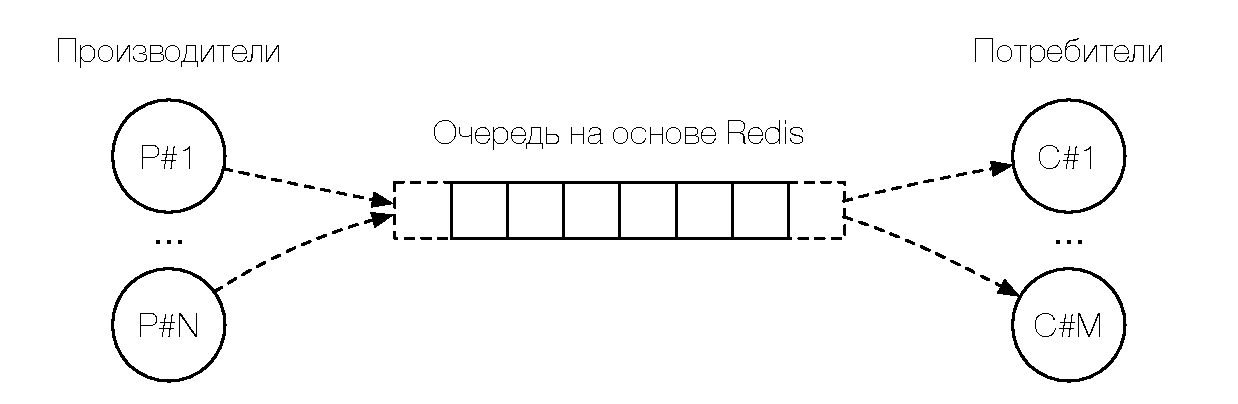
\includegraphics[scale=0.5]{producer-consumer-simple.pdf}
  \end{center}

  \begin{itemize}
    \item Реализована на основе библитеки Kue
    \item Задания сохраняются после перезапуска сервера
    \item Компоненты, работающие с очередью, изолированы
  \end{itemize}
\end{frame}

\begin{frame}{Подготовка к печати}
  \begin{columns}
    \begin{column}{0.4\textwidth}
      \begin{itemize}
        \item Загрузка фотографии в облачное хранилище Amazon S3\\[0.5cm]
        \item Компоновка изображения с помощью \textbf{canvas}\\[0.5cm]
        \item Вызов RPC-функции \texttt{print} печатной станции
      \end{itemize}
    \end{column}

    \begin{column}{0.6\textwidth}
      \begin{center}
        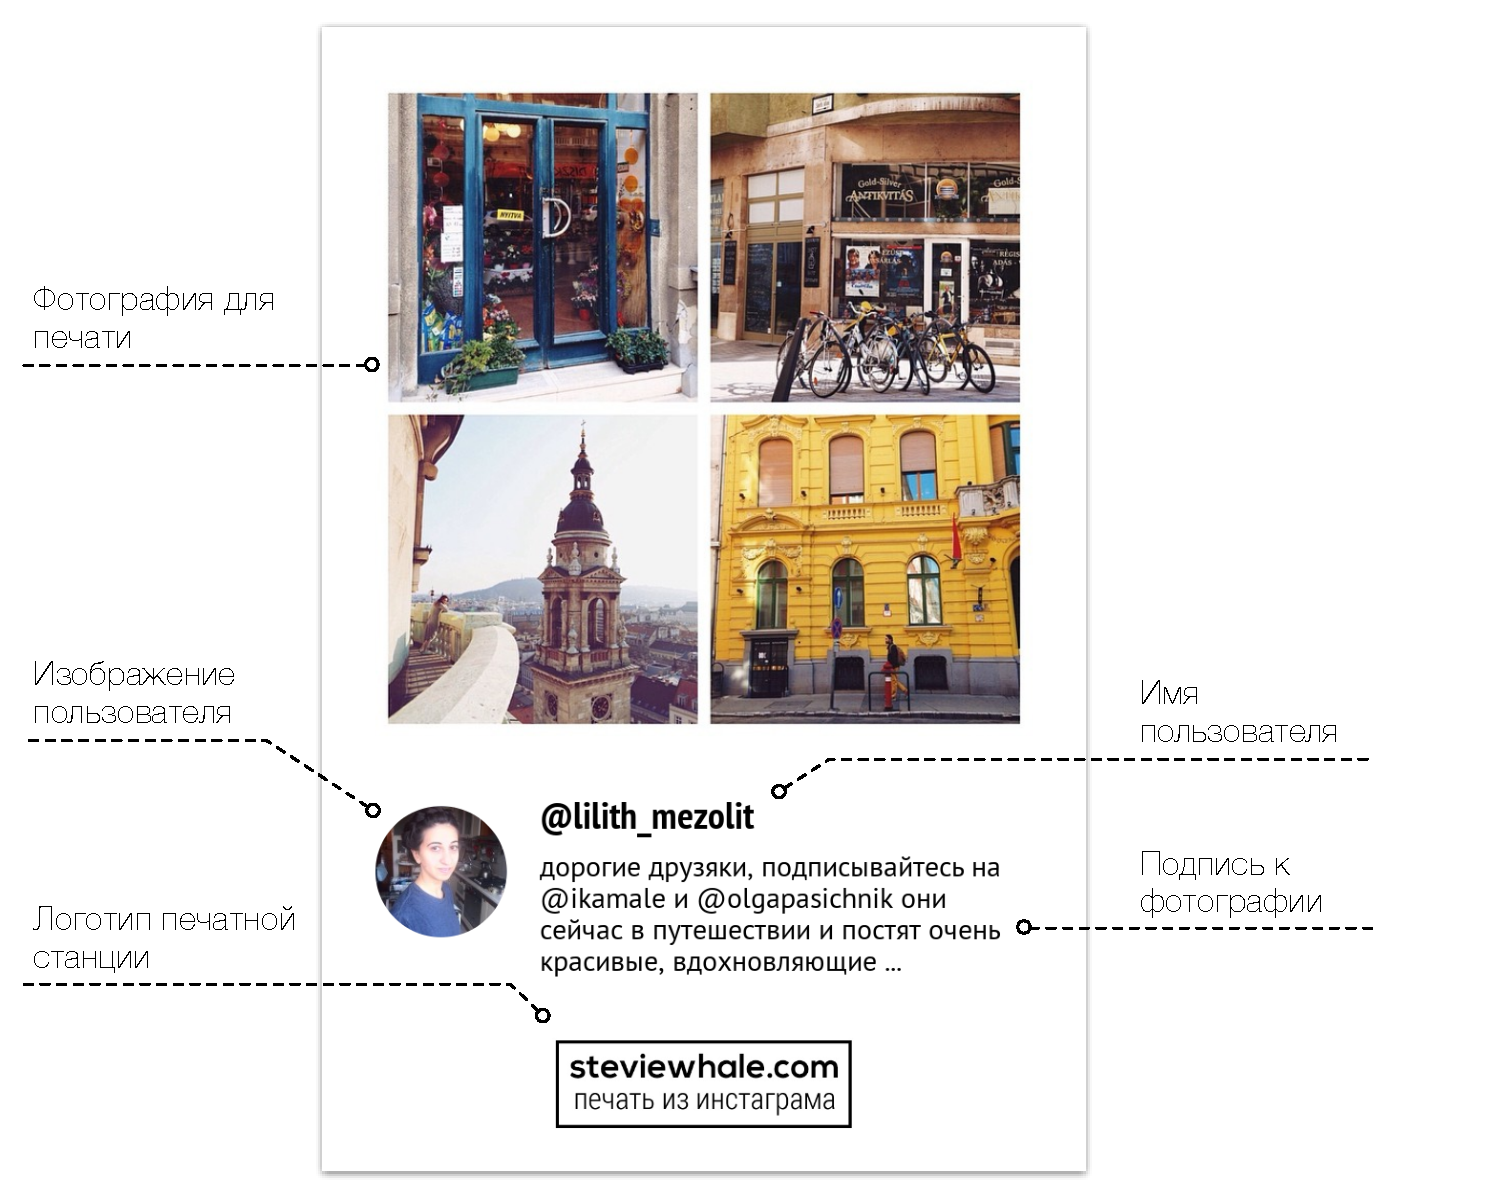
\includegraphics[scale=0.3]{photo-layout.pdf}
      \end{center}
    \end{column}

  \end{columns}
\end{frame}


% С++
\def\CC{{C\nolinebreak[4]\hspace{-.05em}\raisebox{.4ex}{\tiny\bf ++}}}

\begin{frame}{Печать в рамках печатной станции}
    \begin{itemize}
      \item \textbf{cupsidity} --- реализованный модуль на \CC, предоставляющий интерфейс к
        функциям подсистемы печати CUPS в JavaScript.\\[0.5cm]
      \item Модуль опубликован в репозитории пакетов NPM.
    \end{itemize}
\end{frame}


\begin{frame}{Мониторинг статуса задания печати}
  \begin{center}
        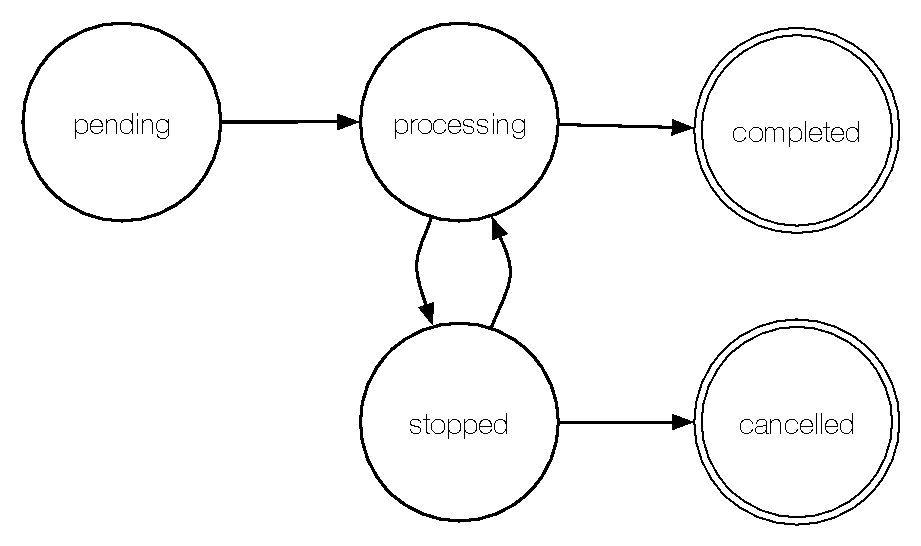
\includegraphics[scale=0.5]{printer-class-simple.pdf}
  \end{center}
  Класс-обертка \texttt{Printer} предосталяет высокоуровневый интерфейс печати, детектируя изменение статуса заданий
  посредством \textbf{cupsidity}.
\end{frame}


\section{Интеграция}
\begin{frame}{Особенности реализации}

  \begin{block}{Контроль версий}
    git, GitHub
  \end{block}

  \begin{block}{Непрерывная интеграция}
    Travis CI
  \end{block}


  \begin{block}{Развертывание}
    Автоматическое развертывание при исполнении команды \texttt{git push}
  \end{block}

\end{frame}


\section{Результаты работы}
\begin{frame}{Полученные результаты}
  \begin{itemize}
    \item Разработана система для моментальной печати фотографий из социальной сети посредством
      удаленных печатных станций.\\[0.4cm]

    \item Опубликован модуль для взаимодействия с подсистемой печати в открытом репозитории пакетов
      NPM.\\[0.4cm]

    \item Полученная система успешно запущена в производство.
  \end{itemize}
\end{frame}

% %%%%%%%%%%%%%%%%%%%%%%%%%%%%%%%%%%%%%%%
% %           Список литературы         %
% %%%%%%%%%%%%%%%%%%%%%%%%%%%%%%%%%%%%%%%
% \begin{frame}
%   \frametitle{Литература}

%   \bibliographystyle{unsrt}
%   \bibliography{../bibliography/sources}
% \end{frame}

\end{document}